\documentclass{bschlangaul-aufgabe}
\bLadePakete{uml,java}
\begin{document}
\bAufgabenMetadaten{
  Titel = {Aufgabe 2},
  Thematik = {PKI-System Lehrer Schüler},
  Referenz = 66116-2016-H.T1-TA2-A2,
  RelativerPfad = Examen/66116/2016/09/Thema-1/Teilaufgabe-2/Aufgabe-2.tex,
  ZitatSchluessel = examen:66116:2016:09,
  BearbeitungsStand = mit Lösung,
  Korrektheit = unbekannt,
  Ueberprueft = {unbekannt},
  Stichwoerter = {UML-Diagramme, Anwendungsfalldiagramm, Klassendiagramm, Implementierung in Java},
  EinzelpruefungsNr = 66116,
  Jahr = 2016,
  Monat = 09,
  ThemaNr = 1,
  TeilaufgabeNr = 2,
  AufgabeNr = 2,
}

\begin{enumerate}

%%
% a)
%%

\item Gegeben sei folgende natürlichsprachliche Spezifikation eines
PKI-Systems:
\index{UML-Diagramme}
\footcite{examen:66116:2016:09}

{
\itshape
Damit der Schüler seinem Lehrer die Hausaufgaben verschlüsselt per
E-Mail übermitteln kann, bedarf es einer entsprechenden Infrastruktur.
Nachdem beide Teilnehmer die notwendige Software installiert haben,
erstellt der Lehrer zunächst ein sogenanntes Schlüsselpaar, bestehend
aus einem „Öffentlichen“ (ÖS) und einem zugehörigen „privaten“ Schlüssel
(PS). Anschließend veröffentlicht der Lehrer seinen ÖS durch Hochladen
auf einen sogenannten Keyserver (Schlüsselverzeichnisdienst). Damit
steht er jedem Schüler zur Verfügung, so dass dieser den ÖS jederzeit
vom Keyserver herunterladen kann. Alternativ kann der Lehrer seinen ÖS
auch direkt (\zB per E-Mail oder USB-Stick) an den Schüler
übermitteln.

Der Schüler kann nun seine Nachricht (\zB seine Lösung) mit dem ÖS
des Lehrers verschlüsseln und mit einer E-Mail versenden. Empfängt der
Lehrer eine solche E-Mail, so kann er (und nur er) mit seinem PS die
Nachricht wieder entschlüsseln. Umgekehrt kann der Lehrer mit seinem PS
beliebige Informationen (\zB die Note) „digital signieren“. Diese
unterschriebenen Daten übermittelt der Lehrer dann zusammen mit der
digitalen Signatur per E-Mail an den Schüler. Der Schüler kann mit dem
ÖS des Lehrers prüfen, ob die übermittelte Nachricht unverändert und
tatsächlich vom unterschreibenden Lehrer stammt.}

Modellieren Sie die in der Spezifikation beschriebenen Anwendungsfälle
zusammen mit den jeweils beteiligten Aktoren in einem Use-Case-Dia\-gramm.
Betrachten Sie den Keyserver zunächst ebenfalls als Aktor, welcher
gegenüber PKI als „externer Vermittler“ auftritt.
\index{Anwendungsfalldiagramm}

%%
% b)
%%

\item Erstellen Sie ein geeignetes Klassendiagramm für das obige PKI.
Berücksichtigen Sie zusätzlich zur verbalen Spezifikation noch folgende
Präzisierungen:
\index{Klassendiagramm}

\begin{enumerate}

%%
% i.
%%

\item Die Schlüssel werden mit einer E-Mail-Adresse „benannt“, damit der
Schüler den richtigen Schlüssel abrufen kann.

%%
% ii.
%%

\item Es gibt genau einen Keyserver; dieser verwaltet aber beliebig
viele Schlüssel. Er bietet die entsprechenden Dienste zum
Veröffentlichen bzw. Abfragen von Schlüsseln an.

%%
% iii.
%%

\item Jeder Lehrer hat höchstens ein Schlüsselpaar, aber jeder Schlüssel
gehört genau einem Lehrer. Der Schüler hingegen kommuniziert mit
mehreren Lehrern und kennt daher mehrere E-Mail-Adressen.

%%
% iv.
%%

\item Eine Nachricht kann (muss aber nicht) eine Signatur oder einen ÖS
als „Anhang“ zusätzlich zum eigentlichen Inhalt (zur Vereinfachung:
String) mit sich führen.

%%
% v.
%%

\item Für das Signieren bzw. Entschlüsseln ist der PS (das zugehörige
Objekt selbst) zuständig. Dafür bekommt er den Inhalt der Nachricht und
gibt entsprechend eine Signatur bzw. den entschlüsselten Inhalt zurück.

%%
% vi.
%%

\item Für das Prüfen der Signatur und das Verschlüsseln ist der ÖS
zuständig. Dazu bekommen die Methoden je nach Bedarf den Inhalt der
Nachricht und die Signatur und liefern einen Wahrheitswert bzw. den
verschlüsselten Inhalt zurück.

\end{enumerate}

%%
% c)
%%

\item Übertragen Sie folgendes UML-Klassendiagramm in Programm-Code
einer gängigen und geeigneten objektorientierten Sprache Ihrer Wahl. Die
Methodenrümpfe dürfen Sie dabei leer lassen (auch wenn das Programm dann
nicht übersetzbar bzw. ausführbar wäre).
\index{Implementierung in Java}

\begin{tikzpicture}
\umlclass[x=0,y=0,type=interface]{IMap}{
}{
  get(key: String): Object\\
  put(key: String, value: Object)
}

\umlclass[x=6,y=0]{MapImpl}{
  \umlstatic{serialVersionUID}: long = 123 \{readonly\}\\
  actualSize: int
}{
  put(key: String, value: Object) MapImpl)\\
  get(key: String): Object
}

\umlclass[x=6,y=-3.5]{MapEntry}{
  key: String\\
  value: Object
}{
  MapEntry(key: String, value: Object)
}

\umlreal{MapImpl}{IMap}
\umlcompo[mult=*,arg=entries]{MapImpl}{MapEntry}
\end{tikzpicture}

\begin{bAntwort}
\bPseudoUeberschrift{Interface „IMap“}
\bJavaExamen{66116}{2016}{09}{pki/IMap}

\bPseudoUeberschrift{Klasse „MapImpl“}
\bJavaExamen{66116}{2016}{09}{pki/MapImpl}

\bPseudoUeberschrift{Klasse „MapEntry“}
\bJavaExamen{66116}{2016}{09}{pki/MapEntry}
\end{bAntwort}

\end{enumerate}

\end{document}
